\documentclass[conference]{IEEEtran}
\IEEEoverridecommandlockouts
\usepackage{cite}
\usepackage{amsmath,amssymb,amsfonts}
\usepackage{graphicx}
\usepackage{booktabs}
\usepackage{algorithm}
\usepackage{algpseudocode}
\usepackage{url}
\graphicspath{{./}}
\def\BibTeX{{\rm B\kern-.05em{\sc i\kern-.025em b}\kern-.08em T\kern-.1667em\lower.7ex\hbox{E}\kern-.125emX}}

\begin{document}

\title{CB-SAFE: Code-Based Post-Quantum Secure\\Aggregation for Byzantine-Robust Federated Learning}

\author{%
\IEEEauthorblockN{Wahiduzzaman Suva}
\IEEEauthorblockA{\textit{Dept.\ of Computer Science and Engineering} \\
\textit{American International University-Bangladesh} \\
Dhaka, Bangladesh \\
26-94088-2@student.aiub.edu}
\and
\IEEEauthorblockN{Esme Moula Chowdhury Abha}
\IEEEauthorblockA{\textit{Dept.\ of Computer Science and Engineering} \\
\textit{American International University-Bangladesh} \\
Dhaka, Bangladesh \\
26-94089-2@student.aiub.edu}}

\maketitle

\begin{abstract}
Federated learning (FL) keeps raw data on-device, yet the transmitted model
updates leak private information, and secure aggregation, which masks individual
updates so the server sees only their sum, has become the standard mitigation.
This creates two open problems. First, the masks rest on classical key exchange
that a quantum computer breaks, and the few post-quantum FL systems are almost
exclusively lattice-based, concentrating systemic risk on a single hardness
assumption. Second, hiding individual updates denies Byzantine-robustness
defenses the visibility they need. We critically review 20 recent high-quality
papers spanning secure aggregation, post-quantum FL, and Byzantine-robust FL, and
show that no existing framework simultaneously provides code-based post-quantum
confidentiality, Byzantine robustness, per-client identification, and scalability.
To close this gap we propose \textbf{CB-SAFE}, a KEM-agnostic secure-aggregation
protocol instantiated with the NIST-selected code-based KEM HQC, robust aggregation
over cluster sums, and \textbf{CB-SAFE+}, a temporal group-testing defense that
identifies hidden attackers from privacy-preserving observations. We detail the
methodology and an evaluation plan over four datasets and three attack families.
\end{abstract}

\begin{IEEEkeywords}
Federated learning, secure aggregation, post-quantum cryptography, code-based KEM,
Byzantine robustness, group testing.
\end{IEEEkeywords}

\section{Introduction}
Federated learning (FL) trains a shared model across many clients without
centralizing their data \cite{mcmahan2017}, but the transmitted updates are not
private: gradient-inversion attacks reconstruct training samples from a single
update \cite{zhu2019}. Secure aggregation closes this channel by ensuring the
server observes only the \emph{sum} of updates, using pairwise masks that cancel on
aggregation \cite{bonawitz2017}. The confidentiality of those masks, however, rests
on key establishment that Shor's algorithm breaks once a cryptographically relevant
quantum computer exists \cite{shor1997}, and traffic recorded today can be decrypted
later. The standard fix replaces classical key exchange with a post-quantum KEM;
nearly all post-quantum FL does so with \emph{lattice} cryptography, concentrating an
entire ecosystem's confidentiality on one assumption. In March~2025 NIST selected
the \emph{code-based} KEM HQC as a diversified backup to the lattice standard
\cite{nistir8545}; that diversity has not yet reached FL.

A second, orthogonal tension is that secure aggregation and Byzantine robustness
pull in opposite directions: hiding individual updates removes exactly the
per-client signal that poisoning defenses rely on. This proposal update
(i)~synthesizes the recent literature across these three areas, (ii)~establishes the
resulting research gap, and (iii)~develops a detailed methodology for CB-SAFE, the
first code-based post-quantum secure-aggregation framework that is also
Byzantine-robust, identifies malicious clients, and scales beyond a fixed small
population.

\section{Literature Review}
The literature relevant to CB-SAFE falls into four themes: secure aggregation,
post-quantum federated learning, Byzantine-robust aggregation, and their intersection.
We review the most pertinent recent work in each and, rather than summarizing studies
individually, compare them critically by what each approach does, how it works, and
where it falls short. Table~\ref{tab:lit} consolidates this comparison.

\subsection{Secure Aggregation}
Bonawitz \emph{et al.}~\cite{bonawitz2017} introduced masking-based secure
aggregation with dropout tolerance via secret-shared seeds; Bell \emph{et
al.}~\cite{bell2020} reduced its quadratic cost to (poly)logarithmic, and
LightSecAgg~\cite{lightsecagg} and SwiftAgg~\cite{swiftagg} further lower
communication with coded one-shot recovery. Flamingo~\cite{flamingo} removes the
per-round setup for the multi-round FL setting. \emph{Critique:} this line steadily
improves efficiency, but every protocol reveals only the aggregate, which can itself
leak information about participants \cite{elkordy2022}, and, crucially, hides the
per-client updates that robustness defenses require. None is post-quantum.

\subsection{Post-Quantum Federated Learning}
PQSF~\cite{pqsf2024} reconstructs masks with lattice secret sharing; Qin and
Xu~\cite{qinxu2025} build single-round aggregation from a lattice key-homomorphic
PRF; a 2026 framework~\cite{byzpqfl2026} pairs reputation-weighted robustness with
lattice-based aggregation; and CQSA~\cite{cqsa2026} performs clustered aggregation on
near-term \emph{quantum hardware}. \emph{Critique:} confidentiality is uniformly
lattice- or quantum-hardware-based; a single lattice cryptanalytic advance would
break the whole class, and most such systems either omit Byzantine robustness or
assume hardware that is not yet deployable. No code-based instantiation exists.

\subsection{Byzantine-Robust Aggregation}
Robust rules replace the mean: Multi-Krum~\cite{blanchard2017}, coordinate-wise
trimmed mean and median~\cite{yin2018}, Bulyan~\cite{bulyan}, and the geometric
median (RFA)~\cite{rfa}. Trust- and detection-based methods add FLTrust
\cite{fltrust}, FLDetector~\cite{fldetector2022}, and the backdoor defense
FLAME~\cite{flame2022}, motivated by strong poisoning attacks~\cite{fang2020}.
\emph{Critique:} all of these operate on \emph{individual}, cleartext updates, the
precise information secure aggregation removes, so they are fundamentally
incompatible with a privacy-preserving pipeline, and coordinate-wise statistics are
provably fragile against amplified poisoning.

\subsection{Robustness Under Secure Aggregation}
The closest works combine both goals. RoFL~\cite{rofl} enforces zero-knowledge
norm/well-formedness proofs on masked updates; EIFFeL~\cite{eiffel} verifies
secret-shared integrity checks; ELSA~\cite{elsa} uses two-server distributed trust
robust to malicious clients; BREA~\cite{brea2021} secret-shares distance
computations; and PriRoAgg~\cite{priroagg2024} adds privacy to robust aggregation.
FedGT~\cite{fedgt} is nearest to our mechanism: it identifies malicious clients by
non-adaptive group testing~\cite{dorfman1943,aldridge2019} over overlapping
secure-aggregation groups. \emph{Critique:} all are classical (pre-quantum);
RoFL/EIFFeL/ELSA \emph{bound or validate} updates rather than identifying attackers;
and FedGT's parity-check code is fixed for a small population ($n\!\le\!31$) and
over-excludes honest clients under amplified attacks.

\begin{table*}[t]
\caption{Critical review of representative prior work across the three themes: what
each line of work does and how, and its key limitation relative to this project.}
\label{tab:lit}
\centering
\footnotesize
\renewcommand{\arraystretch}{1.3}
\begin{tabular}{@{}p{0.19\textwidth} p{0.44\textwidth} p{0.30\textwidth}@{}}
\toprule
\textbf{Study / category} & \textbf{Approach: what they did and how} & \textbf{Key limitation(s)}\\
\midrule
Secure aggregation \cite{bonawitz2017,bell2020,flamingo} &
Mask each client update with pairwise secrets that cancel on summation, so the server
learns only the aggregate; dropout tolerance via secret-shared seeds, with
(poly)logarithmic-overhead and single-server multi-round variants. &
Classical key exchange (not post-quantum); by hiding per-client updates it removes
exactly the signal that robustness defenses need.\\
Coordinate-wise robust rules \cite{blanchard2017,yin2018,bulyan,rfa} &
Replace the mean with trimmed mean, median, Multi-Krum, or the geometric median to
bound the influence of outlier updates on the aggregate. &
Require cleartext per-client updates (incompatible with secure aggregation); provably
fragile to amplified/laundered sign-flip poisoning.\\
Malicious-client detection \cite{fltrust,fldetector2022,flame2022} &
Flag or down-weight suspicious clients using a trusted root, update-consistency over
rounds, or clustering of gradients. &
Inspect individual updates, breaking privacy; classical only; heuristic thresholds an
adaptive attacker can evade.\\
Robustness under secure aggregation \cite{rofl,eiffel,elsa} &
Enforce constraints on \emph{masked} updates via zero-knowledge norm/well-formedness
proofs, verifiable secret sharing, or two-server distributed trust. &
Classical (pre-quantum); \emph{bound or validate} updates rather than identifying
which clients are malicious.\\
Group-testing identification (FedGT) \cite{fedgt} &
Identify malicious clients by non-adaptive group testing over overlapping
secure-aggregation groups, decoded with a per-round BCJR decoder. &
Classical; parity-check code fixed for $n\!\le\!31$ clients; over-excludes honest
clients under laundering.\\
Post-quantum FL \cite{pqsf2024,qinxu2025,byzpqfl2026,cqsa2026} &
Replace classical key exchange with lattice KEMs/secret sharing (or quantum hardware)
for post-quantum confidential aggregation. &
Lattice/quantum-only (monoculture risk); most omit Byzantine robustness; no code-based
instantiation.\\
\textbf{CB-SAFE+ (this work)} &
Code-based (HQC) KEM-agnostic masked cluster aggregation, robust aggregation across
cluster sums, and temporal group testing to identify hidden attackers. &
Unifies code-based post-quantum confidentiality, robustness, per-client
identification, and scaling in a single framework.\\
\bottomrule
\end{tabular}
\end{table*}

\textbf{Synthesis.} Across the literature, confidentiality and robustness have been
advanced largely in isolation: secure-aggregation and post-quantum work protect
privacy but suppress the signal defenses need, while robust-aggregation work assumes
cleartext updates. The handful of systems that reconcile the two remain classical and
either bound updates instead of identifying attackers (RoFL, EIFFeL, ELSA) or, like
FedGT, identify attackers only within a fixed small population, as the limitation
column of Table~\ref{tab:lit} makes clear.

\section{Research Gap and Problem Statement}
\textbf{Gap.} No FL framework simultaneously provides (1)~\emph{code-based}
post-quantum confidentiality (a hedge against lattice-only monoculture), (2)~secure
aggregation, (3)~Byzantine robustness, (4)~explicit per-client identification of
attackers, and (5)~scalability beyond a fixed small client count.
Table~\ref{tab:comp} makes this explicit as a capability matrix: every prior family
misses at least one axis, and only CB-SAFE+ satisfies all six.

\begin{table}[t]
\caption{Capability matrix across six axes. \checkmark = supported, $\times$ = not,
$\sim$ = partial.}
\label{tab:comp}
\centering
\scriptsize
\setlength{\tabcolsep}{3pt}
\begin{tabular}{@{}lcccccc@{}}
\toprule
 & Post- & Code- & Secure & Byz.- & Identi- & Scales\\
Approach & quantum & based & agg. & robust & fies & $N{>}31$\\
\midrule
Secure agg.~\cite{bonawitz2017,bell2020}      & $\times$ & $\times$ & \checkmark & $\times$ & $\times$ & \checkmark\\
Robust rules~\cite{blanchard2017,yin2018}     & $\times$ & $\times$ & $\times$ & \checkmark & $\times$ & \checkmark\\
FLDetector~\cite{fldetector2022}              & $\times$ & $\times$ & $\times$ & \checkmark & \checkmark & \checkmark\\
RoFL/EIFFeL/ELSA~\cite{rofl,eiffel,elsa}      & $\times$ & $\times$ & \checkmark & \checkmark & $\times$ & \checkmark\\
FedGT~\cite{fedgt}                            & $\times$ & $\times$ & \checkmark & \checkmark & \checkmark & $\times$\\
Lattice PQ-FL~\cite{pqsf2024,byzpqfl2026}     & \checkmark & $\times$ & \checkmark & $\sim$ & $\times$ & \checkmark\\
\textbf{CB-SAFE+ (ours)}                      & \checkmark & \checkmark & \checkmark & \checkmark & \checkmark & \checkmark\\
\bottomrule
\end{tabular}
\end{table}

\textbf{Problem statement.} Given $N$ clients of which a fraction $f$ are Byzantine,
train a global model such that (a)~the server learns only aggregate information under
a post-quantum, code-based confidentiality assumption, and (b)~malicious clients are
identified and excluded despite never being observed individually. A key obstacle we
target is a \emph{laundering} effect: averaging poisoned and honest updates within a
privacy cluster turns an amplified sign-flip attack into a plausible-magnitude,
direction-inverted cluster sum that defeats coordinate-wise robust rules, so
robustness must be recovered \emph{without} breaking the privacy that causes it.

\section{Proposed Methodology}
\subsection{Overview and Per-Round Workflow}
CB-SAFE augments standard federated averaging with three protective layers (a
code-based post-quantum masking layer, a clustering layer that trades privacy against
robustness in a controlled way, and a temporal detection layer) while keeping the
server's view limited to cluster-level sums. The end-to-end pipeline is shown in
Fig.~\ref{fig:arch}. Before training, each client performs a \emph{one-time} HQC key
encapsulation to establish long-lived pairwise secrets. Then, in every round~$r$:
(1)~each client trains the global model locally for one epoch and blinds its update
with pairwise masks; (2)~clients are partitioned into $k$ clusters of size~$c$ and
secure aggregation runs \emph{within} each cluster, so the server receives only $k$
cluster sums, never an individual update; (3)~the server applies a robust aggregation
rule \emph{across} those cluster sums to update the global model; and (4)~a
loss/direction probe on each cluster sum feeds a temporal group-testing procedure that
accumulates per-client suspicion and, after a warmup, excludes identified attackers.
Steps~1--4 repeat with a \emph{freshly randomized} clustering every round, which is
exactly what makes attacker identification possible without de-anonymizing any single
client. Algorithm~\ref{alg:round} summarizes the server-side round.

\begin{figure*}[t]
\centering
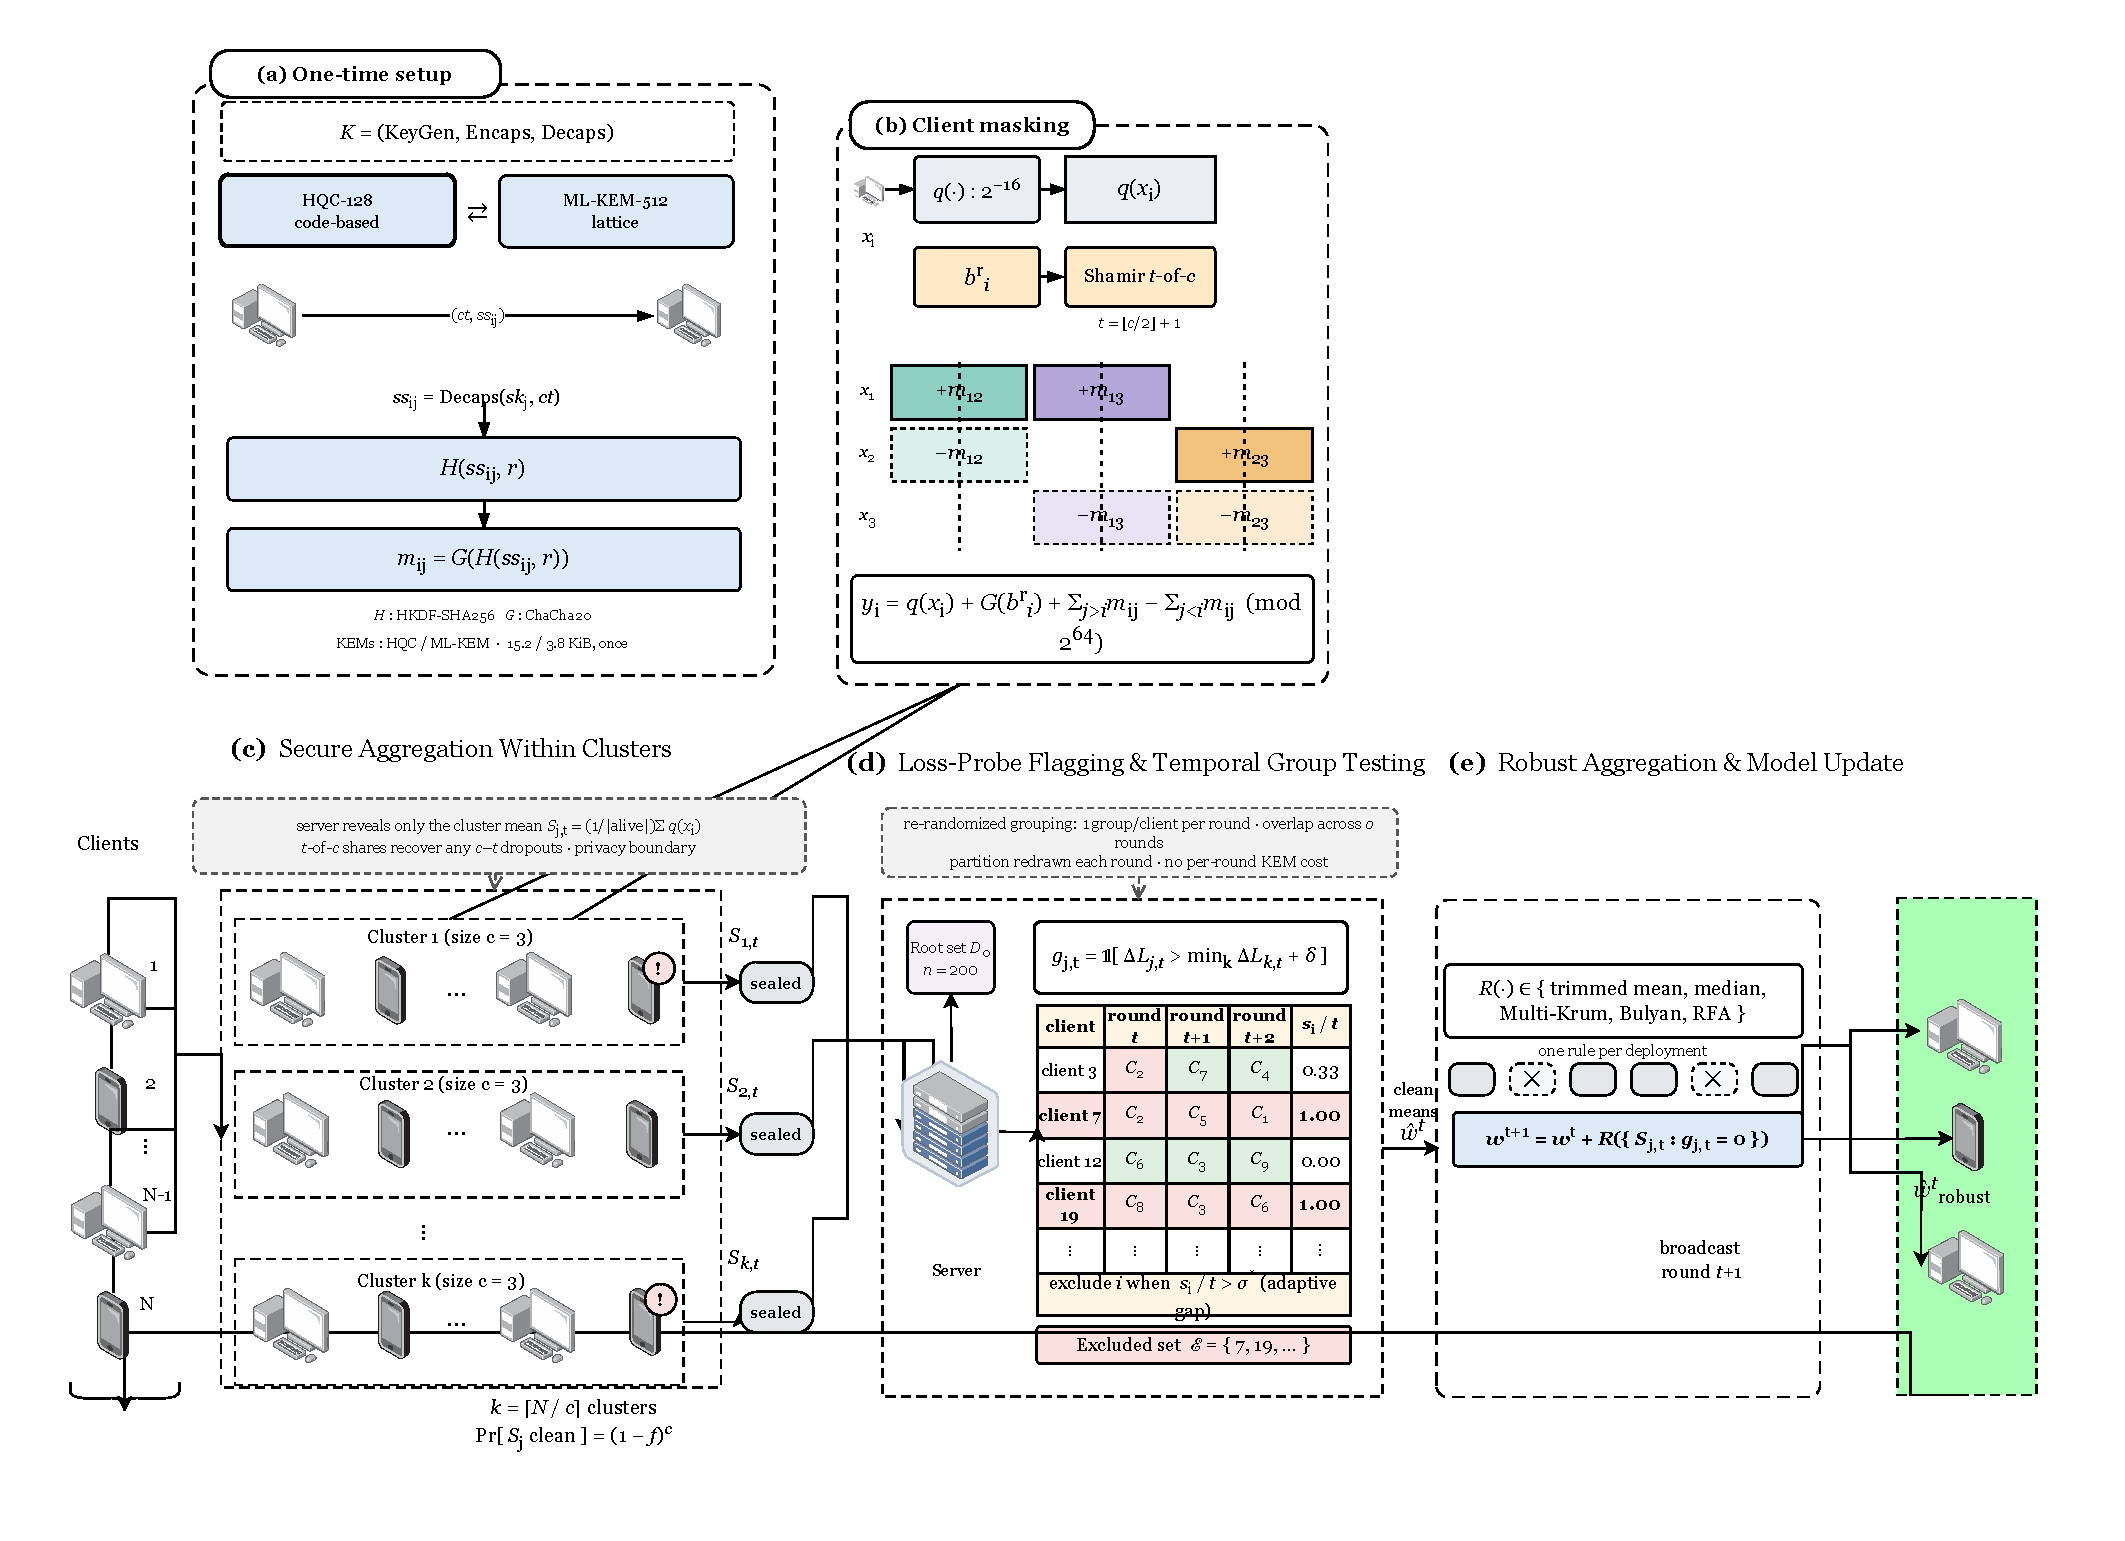
\includegraphics[width=\textwidth]{fig_architecture.pdf}
\caption{CB-SAFE end-to-end pipeline: one-time code-based (HQC) key setup, per-round
masked cluster aggregation, robust aggregation across cluster sums, and CB-SAFE+
temporal group-testing exclusion.}
\label{fig:arch}
\end{figure*}

\subsection{Code-Based Post-Quantum Masked Aggregation}
The confidentiality layer generalizes Bonawitz-style double masking
\cite{bonawitz2017} to run over \emph{any} IND-CCA2 KEM through a KEM-agnostic
interface. Each pair of clients derives a shared secret once, via HQC key
encapsulation; per-round mask seeds are expanded from that secret with HKDF-SHA256 and
realized as ChaCha20 keystreams that cancel exactly when cluster members' updates are
summed, so the server recovers the cluster sum but learns nothing about any single
update. Because encapsulation occurs only at setup, the code-based premium (HQC's
larger keys/ciphertexts and slower operations relative to lattice KEMs) is a
\emph{one-time} cost amortized over all training rounds, while per-round communication
is KEM-independent. Substituting ML-KEM for HQC changes exactly one module, letting us
report both at matched NIST levels~1/3/5 and confirm that the two produce numerically
identical models.

\subsection{Clustering and the Privacy--Robustness Trade-off}
Secure aggregation alone hides individual updates but blinds robust aggregation: a
single global sum cannot be filtered for outliers. CB-SAFE resolves this by
aggregating securely \emph{within} clusters of size~$c$ and applying a robust rule
(trimmed mean, median, or Multi-Krum) \emph{across} the $k$ resulting cluster sums.
This exposes a tunable dial: each client's anonymity set is~$c$, while the probability
that a cluster contains none of the $fN$ attackers decays as $(1-f)^c$. Larger~$c$
strengthens privacy but raises the chance a cluster is contaminated. Critically, we
identify a \emph{laundering} effect: an amplified sign-flip attacker inside a cluster
yields a plausible-magnitude, direction-inverted cluster sum that coordinate-wise
robust rules cannot separate from an honest one. Recovering robustness therefore
requires \emph{identifying} the responsible clients, not merely trimming outliers.

\subsection{CB-SAFE+: Temporal Group-Testing Detection}
CB-SAFE+ turns the per-round cluster sums into a non-adaptive group test spread over
time. Against a small server-held root dataset $\mathcal{D}_0$ (200 samples, disjoint
from all clients), each cluster sum yields a binary flag indicating whether it drives
the model in a harmful direction (rising root loss or inverted gradient). Because the
clustering is re-randomized each round, a fixed attacker is repeatedly placed in
different, overlapping groups; combinatorial (COMP) decoding of the accumulated flags
concentrates suspicion on the clients that are consistently ``defective.'' After a
warmup of $W$ rounds, clients whose suspicion exceeds a threshold~$\tau$ (or an
adaptive gap rule) are excluded for the remainder of training. Because the flags are
post-processing of \emph{already-revealed} cluster sums, CB-SAFE+ adds no
update-content leakage beyond CB-SAFE: attackers are identified without ever being
observed individually.

\begin{algorithm}[t]
\caption{CB-SAFE round $r$ (server view)}
\label{alg:round}
\begin{algorithmic}[1]
\State \textbf{Input:} global model $\theta$; clusters $\{C_j\}_{j=1}^{k}$ of size $c$;
root set $\mathcal{D}_0$; threshold $\tau$; warmup $W$
\For{each client $i$ (in parallel)}
  \State $\delta_i \gets \textsc{LocalTrain}(\theta)$; send \emph{masked} $\delta_i$ within its cluster
\EndFor
\For{each cluster $j$}
  \State server obtains cluster sum $S_j=\sum_{i\in C_j}\delta_i$ \Comment{masks cancel}
  \State $g_j \gets$ loss/direction flag of $S_j$ against $\mathcal{D}_0$
\EndFor
\State $\theta \gets \theta + \textsc{RobustAgg}\big(\{S_j/c\}\big)$ \Comment{trimmed mean / median / Multi-Krum}
\If{$r \ge W$}
  \State update per-client suspicion by COMP decoding of flags $\{g_j\}$ over the
  re-randomized group assignment \Comment{temporal group testing}
  \State exclude clients with suspicion $>\tau$
\EndIf
\State re-randomize clustering for round $r{+}1$
\State \textbf{Output:} updated $\theta$, exclusion set
\end{algorithmic}
\end{algorithm}

\subsection{Datasets, Baselines, and Protocol}
\textbf{Datasets.} CIFAR-10, FashionMNIST, EMNIST (image), and Edge-IIoTset (tabular
IoT intrusion detection), partitioned across $N{=}30$ clients by a
Dirichlet($\alpha{=}0.5$) non-IID split. \textbf{Models.} A 291k-parameter CNN for
images and an MLP for Edge-IIoTset. \textbf{Attacks.} Sign-flip (with amplification),
label-flip, and backdoor, at malicious fractions $f\in\{0.1,0.2,0.3\}$.
\textbf{Baselines.} Undefended mean, trimmed mean, median, Multi-Krum, Bulyan,
geometric median (RFA), FLTrust, and the faithful FedGT BCJR decoder.
\textbf{Environment.} PyTorch~2.5 with liboqs (HQC/ML-KEM) on an NVIDIA RTX~2060;
each configuration is repeated over three seeds and reported as mean$\pm$std.
\textbf{Training/validation/testing.} One local SGD epoch per round for 50 rounds; a
held-out test set measures accuracy each round; a 200-sample server root supports the
loss probe.

\section{Expected Outcomes and Evaluation Plan}
\textbf{Metrics.} (i)~Test accuracy vs.\ round and vs.\ $f$; (ii)~backdoor attack
success rate (ASR, lower is better); (iii)~detection quality (attackers identified
and honest false positives); and (iv)~cryptographic overhead (per-round traffic,
one-time key-setup cost, KEM latency). \textbf{Expected results.} We expect CB-SAFE+
to track the clean-training baseline under sign-flip while coordinate-wise rules
collapse at higher $f$; to match FedGT's attacker identification at a lower
false-positive rate while scaling past its $n\!\le\!31$ limit; and to show that the
code-based premium is a \emph{one-time} cost (a few KiB of key material and a
one-time key-setup latency) that is negligible when amortized over training, i.e.,
post-quantum, code-based confidentiality is affordable in FL. \textbf{Validation.}
Statistical significance will be assessed by paired $t$-tests with Holm correction
across matched (dataset, $f$, seed) cells, and cryptographic equivalence by verifying
that HQC and ML-KEM yield numerically identical models.

\section{Conclusion}
The literature reconciles privacy and robustness only in isolation, and post-quantum
FL remains lattice-bound. This proposal update targets that gap with CB-SAFE, a
KEM-agnostic, code-based post-quantum secure-aggregation framework, and CB-SAFE+, a
temporal group-testing defense that identifies hidden attackers without weakening
privacy. The detailed methodology and evaluation plan above make the design directly
implementable and its claims measurable.

\begin{thebibliography}{00}
\bibitem{mcmahan2017} B.\ McMahan, E.\ Moore, D.\ Ramage, S.\ Hampson, and
B.\ A.\ y~Arcas, ``Communication-efficient learning of deep networks from
decentralized data,'' in \emph{Proc.\ AISTATS}, 2017, pp.\ 1273--1282.
\bibitem{zhu2019} L.\ Zhu, Z.\ Liu, and S.\ Han, ``Deep leakage from gradients,''
in \emph{Proc.\ NeurIPS}, 2019, pp.\ 14747--14756.
\bibitem{bonawitz2017} K.\ Bonawitz \emph{et al.}, ``Practical secure aggregation
for privacy-preserving machine learning,'' in \emph{Proc.\ ACM CCS}, 2017,
pp.\ 1175--1191.
\bibitem{bell2020} J.\ H.\ Bell, K.\ A.\ Bonawitz, A.\ Gasc\'on, T.\ Lepoint, and
M.\ Raykova, ``Secure single-server aggregation with (poly)logarithmic overhead,''
in \emph{Proc.\ ACM CCS}, 2020, pp.\ 1253--1269.
\bibitem{lightsecagg} J.\ So \emph{et al.}, ``LightSecAgg: A lightweight and
versatile design for secure aggregation in federated learning,'' in
\emph{Proc.\ MLSys}, 2022, pp.\ 694--720.
\bibitem{swiftagg} T.\ Jahani-Nezhad, M.\ A.\ Maddah-Ali, S.\ Li, and G.\ Caire,
``SwiftAgg: Communication-efficient and dropout-resistant secure aggregation for
federated learning with worst-case security guarantees,'' in \emph{Proc.\ IEEE
ISIT}, 2022, pp.\ 103--108.
\bibitem{flamingo} Y.\ Ma, J.\ Woods, S.\ Angel, A.\ Polychroniadou, and T.\ Rabin,
``Flamingo: Multi-round single-server secure aggregation with applications to private
federated learning,'' in \emph{Proc.\ IEEE Symp.\ Security and Privacy (S\&P)}, 2023,
pp.\ 477--496.
\bibitem{elkordy2022} A.\ R.\ Elkordy, J.\ Zhang, Y.\ H.\ Ezzeldin, K.\ Psounis,
and S.\ Avestimehr, ``How much privacy does federated learning with secure
aggregation guarantee?,'' \emph{Proc.\ Privacy Enhancing Technol.}, 2022,
pp.\ 510--526.
\bibitem{pqsf2024} X.\ Zhang, H.\ Deng, R.\ Wu, J.\ Ren, and Y.\ Ren, ``PQSF:
Post-quantum secure privacy-preserving federated learning,'' \emph{Sci.\ Rep.},
vol.\ 14, Art.\ no.\ 23553, 2024.
\bibitem{qinxu2025} X.\ Qin and R.\ Xu, ``Efficient post-quantum cross-silo
federated learning based on key homomorphic pseudo-random function,''
\emph{Mathematics}, vol.\ 13, no.\ 9, Art.\ no.\ 1404, 2025.
\bibitem{byzpqfl2026} ``Byzantine-robust federated learning framework with
post-quantum secure aggregation for real-time threat intelligence sharing in
critical IoT infrastructure,'' arXiv:2601.01053, 2026.
\bibitem{cqsa2026} ``CQSA: Byzantine-robust clustered quantum secure aggregation in
federated learning,'' arXiv:2602.22269, 2026.
\bibitem{blanchard2017} P.\ Blanchard, E.\ M.\ El Mhamdi, R.\ Guerraoui, and
J.\ Stainer, ``Machine learning with adversaries: Byzantine tolerant gradient
descent,'' in \emph{Proc.\ NeurIPS}, 2017, pp.\ 119--129.
\bibitem{yin2018} D.\ Yin, Y.\ Chen, R.\ Kannan, and P.\ Bartlett,
``Byzantine-robust distributed learning: Towards optimal statistical rates,'' in
\emph{Proc.\ ICML}, 2018, pp.\ 5650--5659.
\bibitem{bulyan} E.\ M.\ El Mhamdi, R.\ Guerraoui, and S.\ Rouault, ``The hidden
vulnerability of distributed learning in Byzantium,'' in \emph{Proc.\ ICML}, 2018,
pp.\ 3521--3530.
\bibitem{rfa} K.\ Pillutla, S.\ M.\ Kakade, and Z.\ Harchaoui, ``Robust aggregation
for federated learning,'' \emph{IEEE Trans.\ Signal Process.}, vol.\ 70,
pp.\ 1142--1154, 2022.
\bibitem{fltrust} X.\ Cao, M.\ Fang, J.\ Liu, and N.\ Z.\ Gong, ``FLTrust:
Byzantine-robust federated learning via trust bootstrapping,'' in \emph{Proc.\ NDSS},
2021.
\bibitem{fldetector2022} Z.\ Zhang, X.\ Cao, J.\ Jia, and N.\ Z.\ Gong,
``FLDetector: Defending federated learning against model poisoning attacks via
detecting malicious clients,'' in \emph{Proc.\ ACM KDD}, 2022, pp.\ 2545--2555.
\bibitem{flame2022} T.\ D.\ Nguyen \emph{et al.}, ``FLAME: Taming backdoors in
federated learning,'' in \emph{Proc.\ USENIX Security}, 2022, pp.\ 1415--1432.
\bibitem{fang2020} M.\ Fang, X.\ Cao, J.\ Jia, and N.\ Z.\ Gong, ``Local model
poisoning attacks to Byzantine-robust federated learning,'' in \emph{Proc.\ USENIX
Security}, 2020, pp.\ 1605--1622.
\bibitem{rofl} H.\ Lycklama, L.\ Burkhalter, A.\ Viand, N.\ K\"uchler, and A.\ Hithnawi,
``RoFL: Robustness of secure federated learning,'' in \emph{Proc.\ IEEE Symp.\ Security
and Privacy (S\&P)}, 2023, pp.\ 453--476.
\bibitem{eiffel} A.\ Roy~Chowdhury, C.\ Guo, S.\ Jha, and L.\ van~der~Maaten,
``EIFFeL: Ensuring integrity for federated learning,'' in \emph{Proc.\ ACM CCS}, 2022,
pp.\ 2535--2549.
\bibitem{elsa} M.\ Rathee, C.\ Shen, S.\ Wagh, and R.\ A.\ Popa, ``ELSA: Secure
aggregation for federated learning with malicious actors,'' in \emph{Proc.\ IEEE Symp.\
Security and Privacy (S\&P)}, 2023, pp.\ 1961--1979.
\bibitem{brea2021} J.\ So, B.\ G\"uler, and A.\ S.\ Avestimehr,
``Byzantine-resilient secure federated learning,'' \emph{IEEE J.\ Sel.\ Areas
Commun.}, vol.\ 39, no.\ 7, pp.\ 2168--2181, 2021.
\bibitem{priroagg2024} S.\ Hou, S.\ Li, T.\ Jahani-Nezhad, and G.\ Caire, ``PriRoAgg:
Achieving robust model aggregation with minimum privacy leakage for federated
learning,'' \emph{IEEE Trans.\ Inf.\ Forensics Security}, 2024.
\bibitem{fedgt} M.\ Xhemrishi, J.\ \"Ostman, A.\ Wachter-Zeh, and A.\ Graell~i~Amat,
``FedGT: Identification of malicious clients in federated learning with secure
aggregation,'' \emph{IEEE Trans.\ Inf.\ Forensics Security}, vol.\ 20,
pp.\ 2577--2592, 2025.
\bibitem{dorfman1943} R.\ Dorfman, ``The detection of defective members of large
populations,'' \emph{Ann.\ Math.\ Stat.}, vol.\ 14, no.\ 4, pp.\ 436--440, 1943.
\bibitem{aldridge2019} M.\ Aldridge, O.\ Johnson, and J.\ Scarlett, ``Group
testing: An information theory perspective,'' \emph{Found.\ Trends Commun.\ Inf.\
Theory}, vol.\ 15, no.\ 3--4, pp.\ 196--392, 2019.
\bibitem{shor1997} P.\ W.\ Shor, ``Polynomial-time algorithms for prime
factorization and discrete logarithms on a quantum computer,'' \emph{SIAM
J.\ Comput.}, vol.\ 26, no.\ 5, pp.\ 1484--1509, 1997.
\bibitem{nistir8545} National Institute of Standards and Technology, ``Status report
on the fourth round of the NIST post-quantum cryptography standardization process,''
NIST IR 8545, Mar.\ 2025.
\bibitem{edgeiiot} M.\ A.\ Ferrag, O.\ Friha, D.\ Hamouda, L.\ Maglaras, and
H.\ Janicke, ``Edge-IIoTset: A new comprehensive realistic cyber security dataset
of IoT and IIoT applications for centralized and federated learning,'' \emph{IEEE
Access}, vol.\ 10, pp.\ 40281--40306, 2022.
\end{thebibliography}

\end{document}
